\documentclass{standalone}
\usepackage{pgfplots}
\pgfplotsset{compat=1.17}

\begin{document}

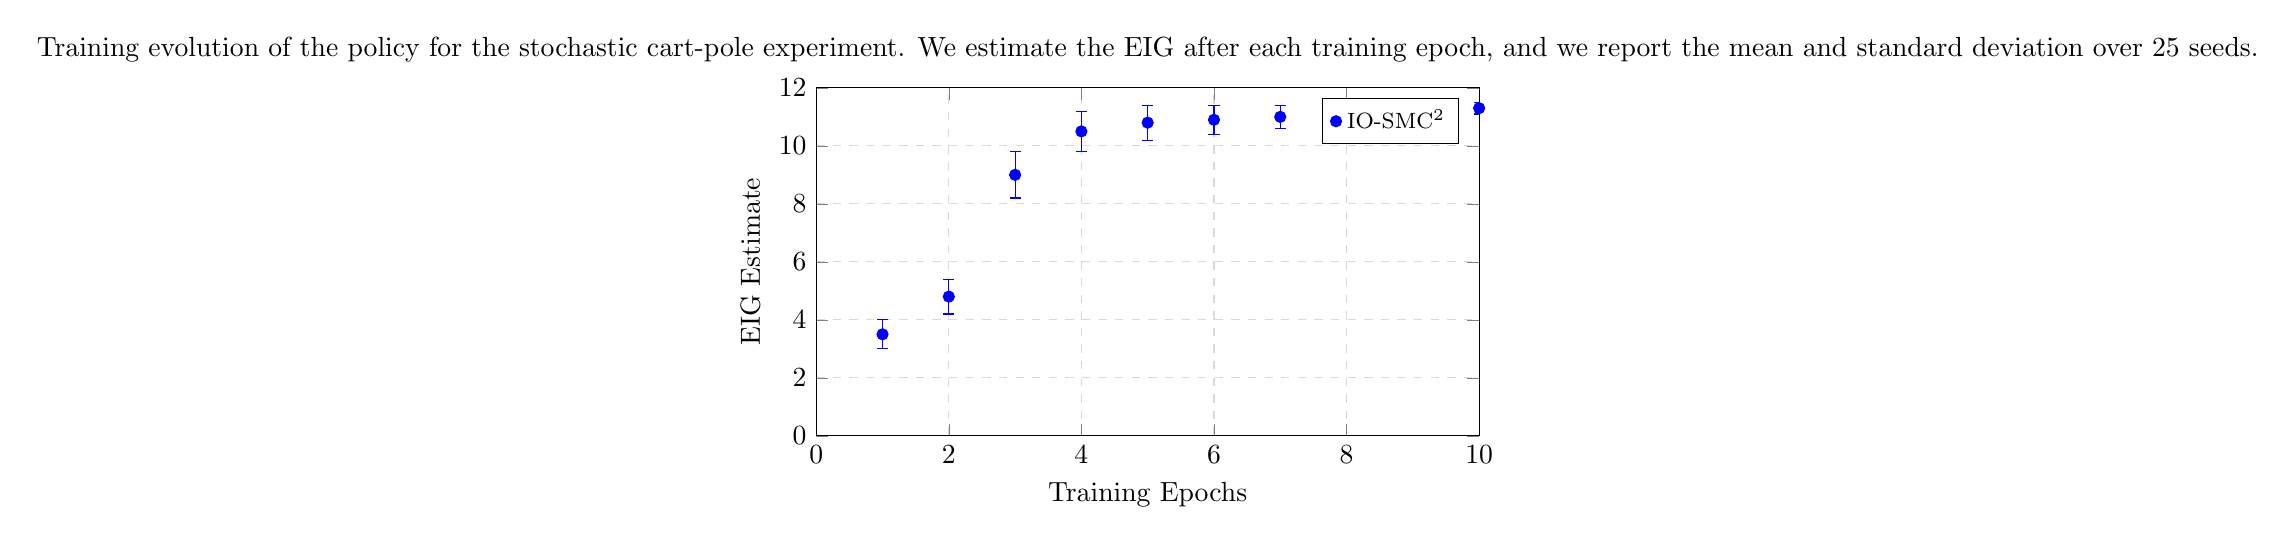
\begin{tikzpicture}
    \begin{axis}[
        title={Training evolution of the policy for the stochastic cart-pole experiment. We estimate the EIG after each training epoch, and we report the mean and standard deviation over 25 seeds.},
        xlabel={Training Epochs},
        ylabel={EIG Estimate},
        xmin=0, xmax=10,
        ymin=0, ymax=12,
        xtick={0,2,4,6,8,10},
        ytick={0,2,4,6,8,10,12},
        grid=major,
        grid style={dashed, gray!30},
        legend pos=north east,
        legend cell align=left,
        legend style={font=\footnotesize},
        width=10cm,
        height=6cm,
        enlargelimits=false,
    ]

    % Data points and error bars
    \addplot+[only marks, mark options={mark=*, solid, fill=blue}, error bars/.cd, y dir=both, y explicit]
        coordinates {
            (1, 3.5) +- (0, 0.5)
            (2, 4.8) +- (0, 0.6)
            (3, 9.0) +- (0, 0.8)
            (4, 10.5) +- (0, 0.7)
            (5, 10.8) +- (0, 0.6)
            (6, 10.9) +- (0, 0.5)
            (7, 11.0) +- (0, 0.4)
            (8, 11.1) +- (0, 0.3)
            (9, 11.2) +- (0, 0.3)
            (10, 11.3) +- (0, 0.2)
        };
    \addlegendentry{IO-SMC$^2$}

    \end{axis}
\end{tikzpicture}

\end{document}